\documentclass[letterpaper,10pt,titlepage]{article}

\usepackage{graphicx}                                        

\usepackage{amssymb}                                         
\usepackage{amsmath}                                         
\usepackage{amsthm}                                       

\usepackage{alltt}                                           
\usepackage{float}
\usepackage{color}

\usepackage{url}

\usepackage{balance}
\usepackage[TABBOTCAP, tight]{subfigure}
\usepackage{enumitem}

\usepackage{pstricks, pst-node}

\usepackage{verbatim}

\usepackage{geometry}
\geometry{textheight=10in, textwidth=7.5in}

%random comment

\newcommand{\cred}[1]{{\color{red}#1}}
\newcommand{\cblue}[1]{{\color{blue}#1}}

\usepackage{hyperref}

\def\name{Geoffrey Corey}

%pull in the necessary preamble matter for pygments output
\input{pygments.tex}

%% The following metadata will show up in the PDF properties
\hypersetup{
  colorlinks = true,
  urlcolor = black,
  pdfauthor = {\name},
  pdfkeywords = {cs311 ``operating systems'' python sockets},
  pdftitle = {CS 311 Project 3: Sockets and python},
  pdfsubject = {CS 311 Project 5},
  pdfpagemode = UseNone
}

\parindent = 0.0 in
\parskip = 0.2 in

\begin{document}
\section{Design}
\label{System Design & Deviations}

\subsection{The Design}
\label{DesingProcess}
The overall design of my system was based upon a simple python echo server with input multiplexing. Most of the time spent was figuring out the best way to use the server and then convert it over to fit the requirements of the project. Firgure \ref{overflow} shows the more detailed design spec.
\begin{figure}[ht!]
\centering
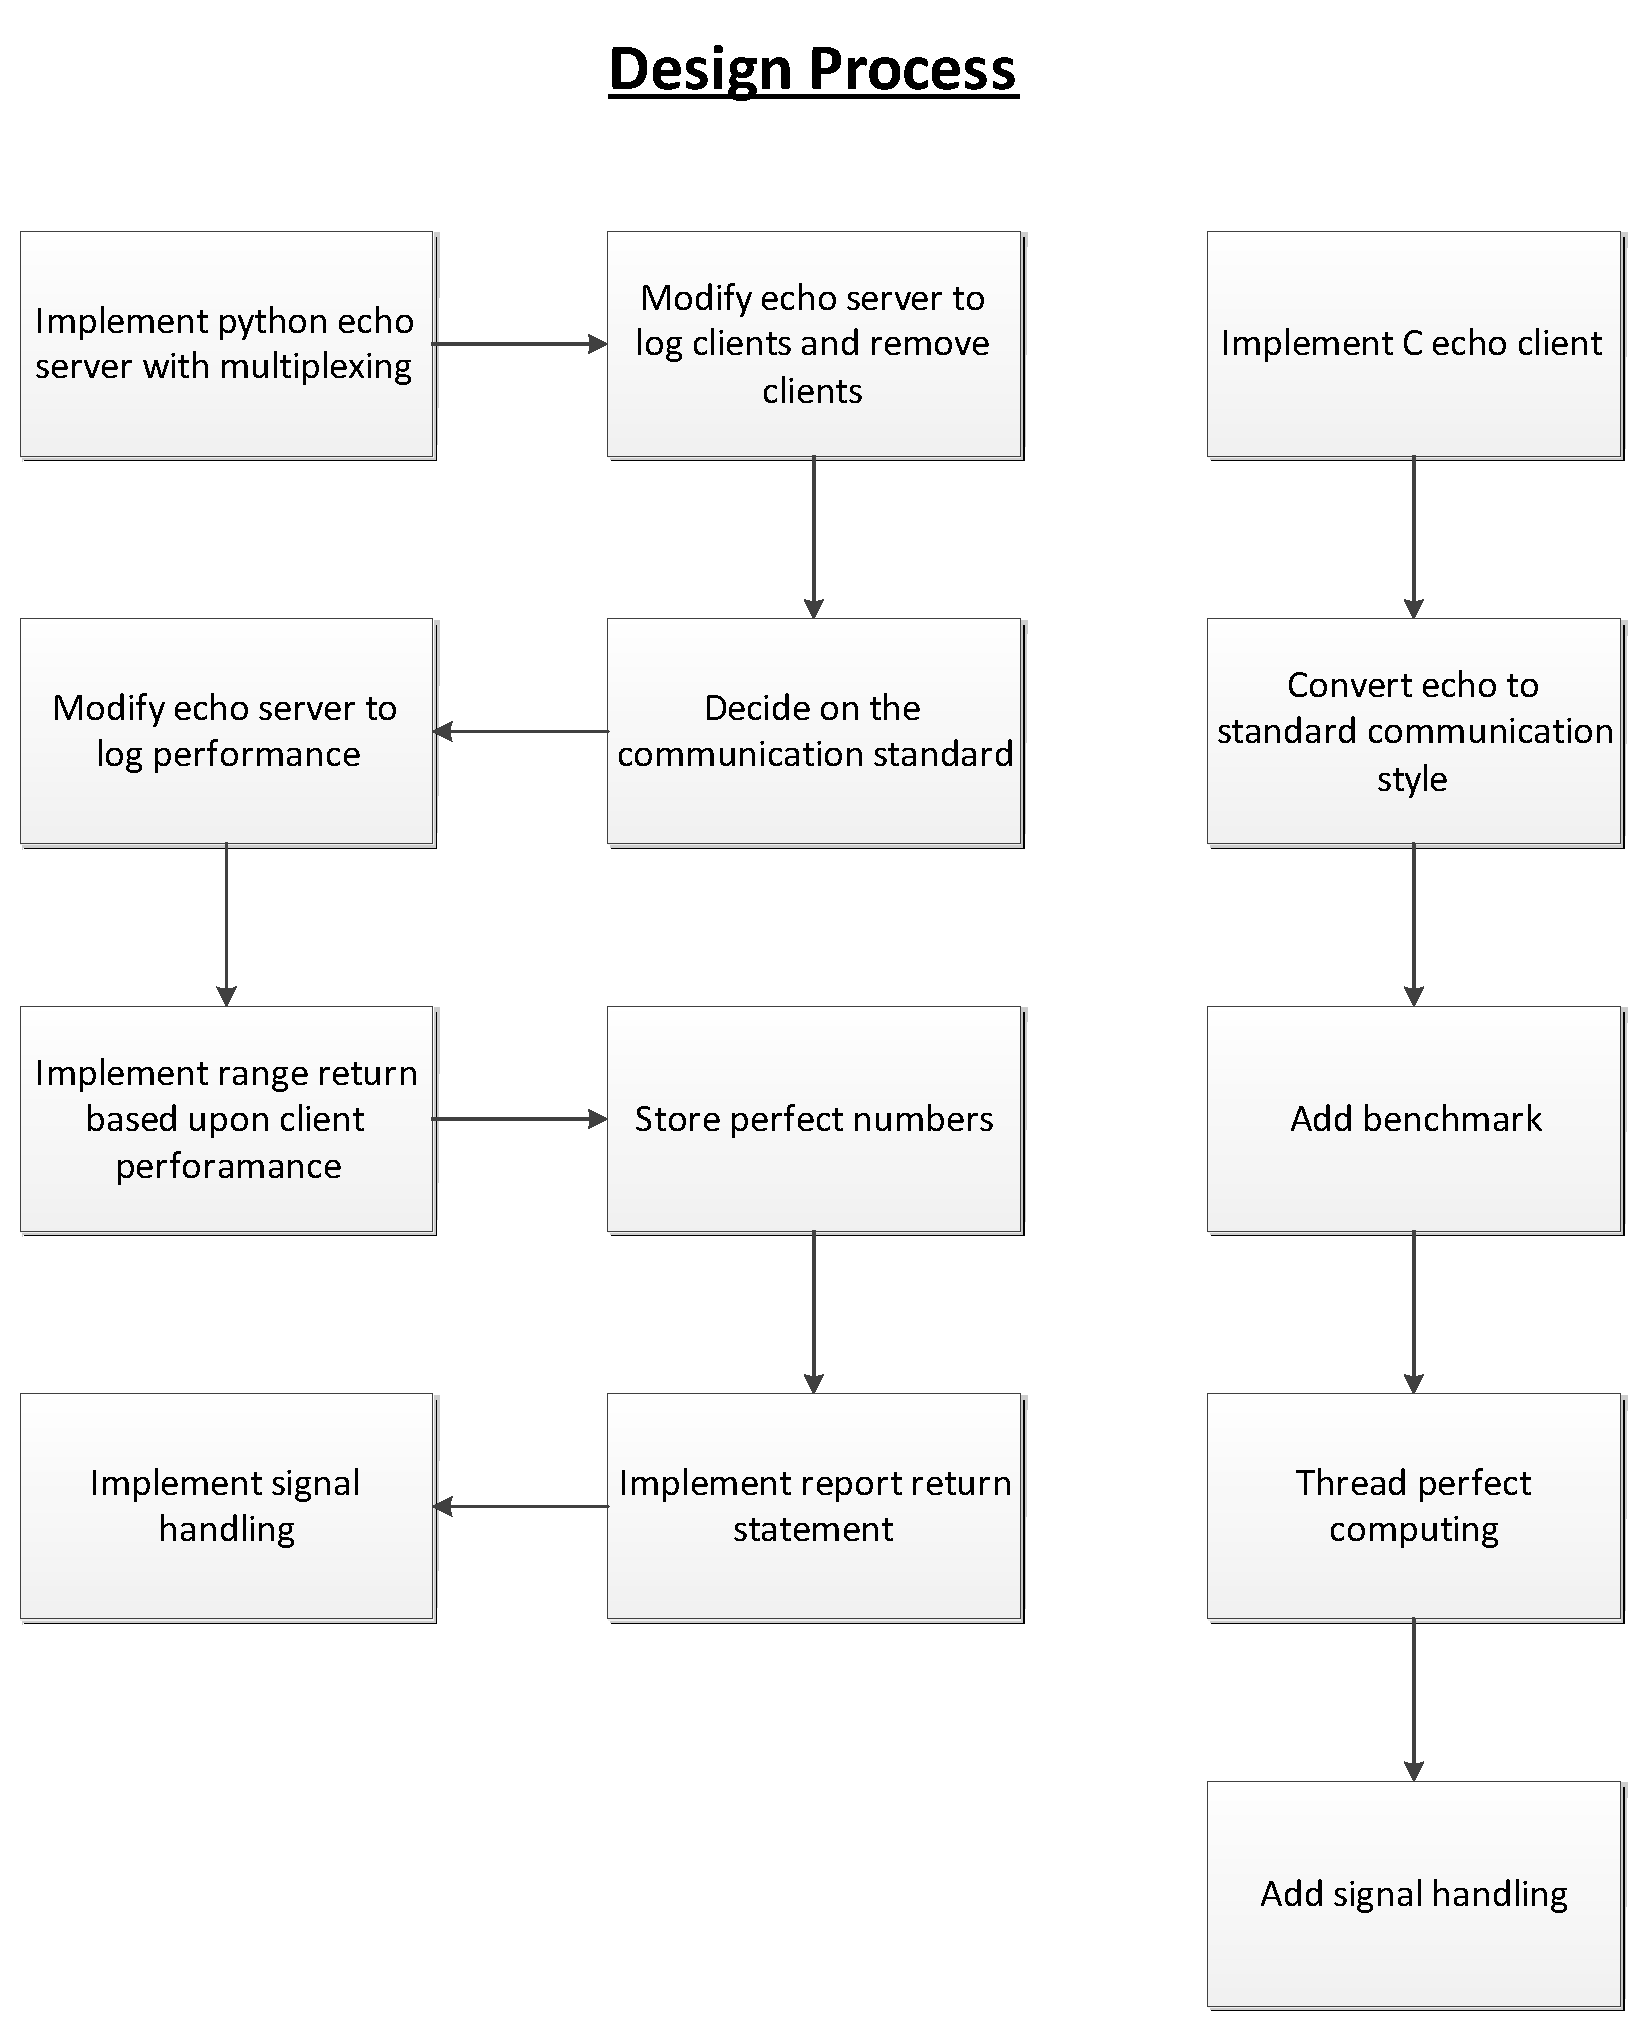
\includegraphics[width=90mm]{HW5Design.eps}
\caption{Outline of the system design}
\label{overflow}
\end{figure}

\subsection{The Deviations}
\label{Deviations}
The only real place that deviated from the original design was how to handle the kill signal. Due to time and the way the original server was designed, adding in the handling of the kill signal from report would have required a redesign of the server.
\section{History}
\label{myar Revision History}
\input{log.txt}

\section{Challenges}
\label{Overcoming Project challenges}
One of the largest obstacles on this assignment was deciding how to setup the server, followed by the communications standard to beused. The largest percentage of time was spent trying to decide how the server was going to work.

\section{Questions}
\label{Project Quesions}
\subsection{The Point of the Assignment}
\label{Point}
The point of this assignment was to learn how to use sockets, how to use network communication, and how to define how to communicate over a network.
\subsection{Quality Assurance}
\label{QA}
When testing this client/server system, I initianted upwards of 7 compute processes on 1 manage process running on a local ARM powered NAS. The reported perfect number were checked against the first 8 or so reported by WolfRamAlpha.
\subsection{What Did You Learn?}
\label{Learned}
From this assignment, I learned the importance of double checking each peice of the system design to make sure it is implmented properly and correctly, as well as how to make each function as light as possible.


%input the pygmentized output of mt19937ar.c, using a (hopefully) unique name
%this file only exists at compile time. Feel free to change that.
\section{Code}
\label{myar Source Code}

\subsection{compute.h}
\label{Compute Header}
\input{__compute.h.tex}

\subsection{compute.c}
\label{Compute}
\input{__compute.c.tex}

\subsection{manage.py}
\label{Manage Server}
\input{__manage.py.tex}

\subsection{report.py}
\label{Report Clinet}
\input{__report.py.tex}

\section{History}
\end{document}
